\problemname{LHC}
For your latest top-secret experiment, you will need a large quantity of Higgs bosons. To obtain
these elusive particles, you will need to build a large hadron collider, a long circular tunnel that
you can use to accelerate particles and smash them into each other.

You already have access to an extensive network of tunnels, which is guaranteed to be connected
and free of cyclic paths. In other words, the existing tunnels form a tree structure. This system can
be represented by $N$ junctions, labelled 1 through $N$, connected by $N - 1$ tunnels, each of which
connects two junctions. Tunnels can be traversed in either direction (i.e., if there is a junction from
a to b, that junction also goes from b to a).

By adding exactly one tunnel to the network, you can create a cyclic path, which you will use to
build your large hadron collider. You wish to form the longest possible collider in this way, where
we define length as the number of tunnels in a cycle. Also, you would like to compute the number of
ways to do this– that is, the number of distinct pairs of junctions such that adding a tunnel
between them forms a cycle of maximum length.

For example, in the following network, we can form a collider of length 4 by building a tunnel
between junctions 1 and 5, or between 2 and 5:
\begin{figure}[h]
    \begin{center}
    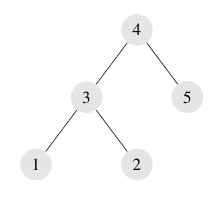
\includegraphics[width=0.4\textwidth]{lhc}
    \end{center}
\end{figure}

\section*{Input}
The first line of each test case will contain $N$ $(3 \le N \le 400\,000)$, the number of junctions.
The next $N - 1$ lines will each contain two space-separated integers $i$ and $j$, indicating that there
istunnel between junctions $i$ and $j$ $(1 \le i, j \le N)$.

\section*{Output}
The output should consist of a single line with two space-separated integers: the length of the
longest possible collider, and the number of ways to achieve that length.

For partial credit you may assume $N \le 5 000$.
